\clearpage
\section{Original mission evidence}
\label{appendix:mission-source-evidence}

These excerpts retain the original content, colours and markings.

\begin{figure}[htbp]
\centering
\small
\textbf{(a) Measured nominal demand, presentation p.~9}\par\smallskip
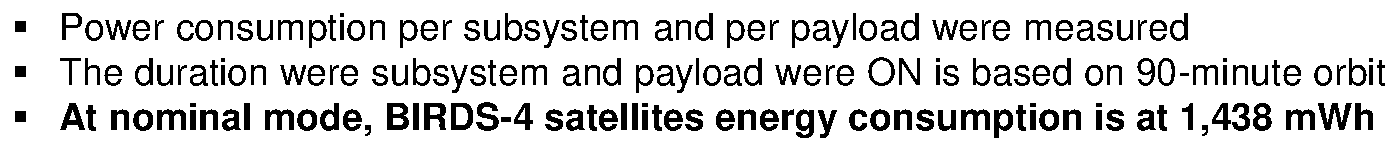
\includegraphics[width=\linewidth]{fig/eps-case-studies/birds-demand.pdf}
\par\bigskip
\textbf{(b) Low-beta generation and losses, presentation p.~8}\par\smallskip
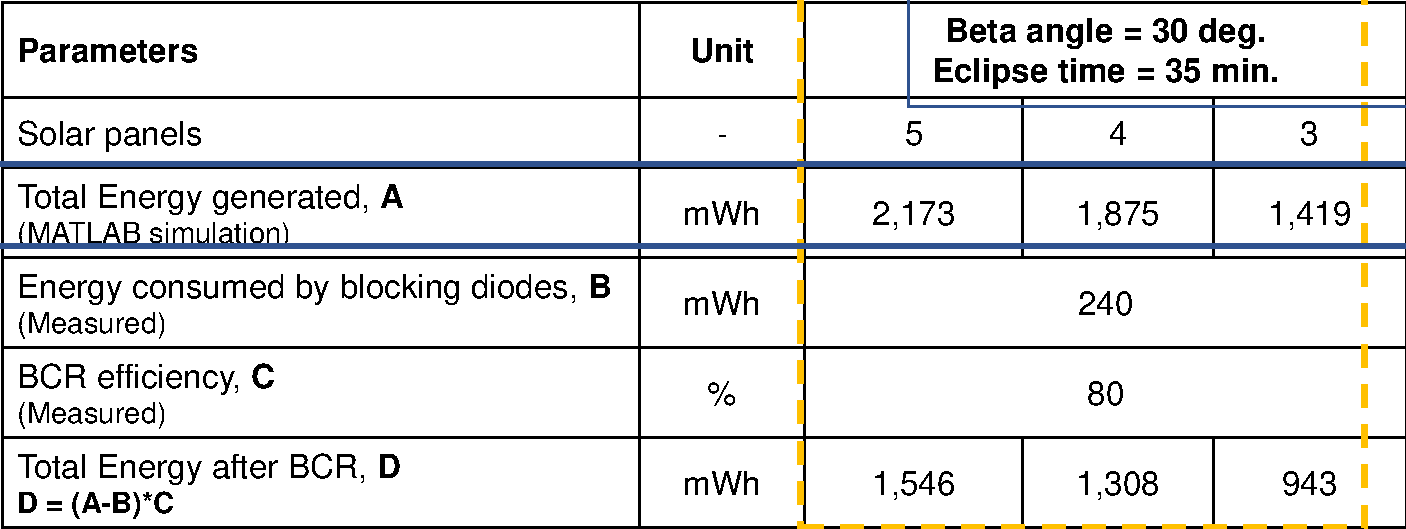
\includegraphics[width=\linewidth]{fig/eps-case-studies/birds-generation.pdf}
\caption[Published BIRDS power budget excerpts.]{Excerpts reproduced (cropped) from Hari Ram Shrestha's BIRDS power budget, LaSEINE, Kyushu Institute of Technology \citep[pp.~8--9]{shrestha2022birds4powerbudget}. The 1.438~Wh demand supplies the MOP-11 requirement. The five-panel generation and loss entries give $(2.173-0.240)0.80=1.5464$~Wh, compared with the printed 1.546~Wh in MOP-11 and MOP-14a. The separate 35-minute eclipse value fixes the MOP-11 sunlight duration.}
\label{fig:source-birds-budget}
\end{figure}
\clearpage

\begin{figure}[p]
\centering
\small
\textbf{(a) Generation, storage and standby demand}\par\smallskip
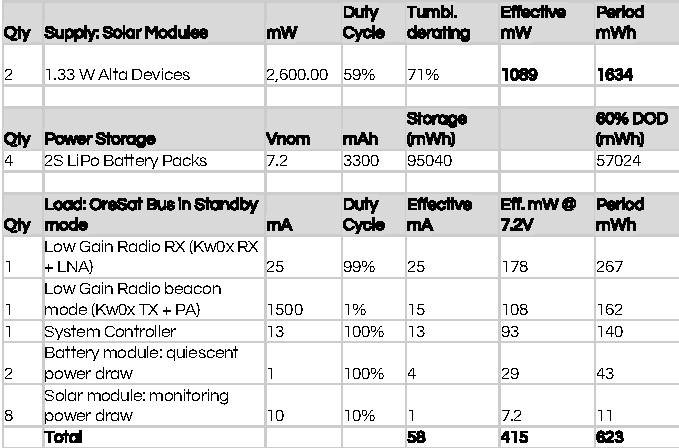
\includegraphics[width=0.92\linewidth]{fig/eps-case-studies/oresat-supply-storage-standby.pdf}
\par\smallskip
\textbf{(b) Live-pass demand}\par\smallskip
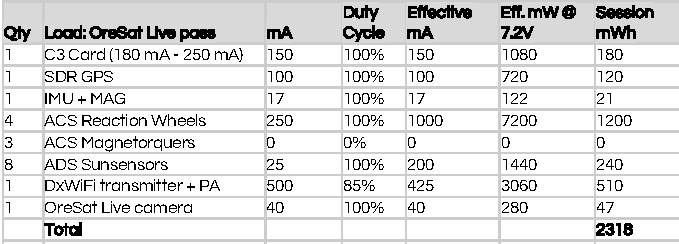
\includegraphics[width=0.92\linewidth]{fig/eps-case-studies/oresat-live.pdf}
\par\smallskip
\textbf{(c) Published pass reserve}\par\smallskip
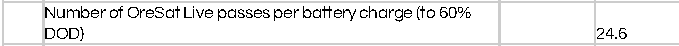
\includegraphics[width=0.92\linewidth]{fig/eps-case-studies/oresat-reserve.pdf}
\caption[Published OreSat power budget excerpts.]{Numerical columns reproduced (cropped) from the OreSat Project's 2019 power budget, Portland State Aerospace Society \citep[pp.~1--2]{oresat2019powerbudget}. The source repository uses the \href{https://github.com/oresat/oresat.github.io/blob/0d879a503be4a6d48e849f3088524c2748503640/LICENSE}{GNU General Public License version 2}. The notes column is omitted. MOP-11 adds the 0.623~Wh standby orbit and 2.318~Wh Live session for its baseline. The published 24.6-pass reserve supplies the stricter storage check. Four 3300~mAh 2S packs and Alta modules belong to this earlier design, separate from the later Tenergy/XTE-SF comparison. The generation row also supplies the MOP-14a budget benchmark.}
\label{fig:source-oresat-budget}
\end{figure}
\clearpage

\begin{figure}[htbp]
\centering
\begin{minipage}[t]{0.47\linewidth}
\centering\small
\textbf{(a) BIRDS battery report}\par\smallskip
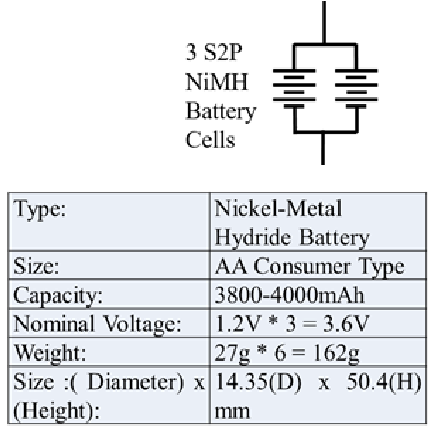
\includegraphics[width=\linewidth]{fig/eps-case-studies/birds-battery-configuration.pdf}
\end{minipage}\hfill
\begin{minipage}[t]{0.49\linewidth}
\centering\small
\textbf{(b) OreSat 2021 account}\par\smallskip
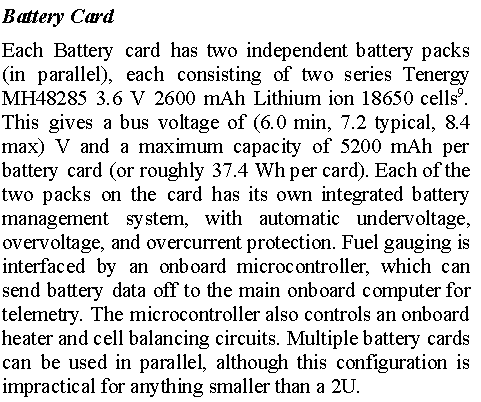
\includegraphics[width=\linewidth]{fig/eps-case-studies/oresat-battery-configuration.pdf}
\end{minipage}
\caption[Published battery arrangements and ratings.]{Battery excerpts reproduced (cropped) from (a) the BIRDS-4 Project, copyright 2021 Kyushu Institute of Technology, \href{https://github.com/BIRDSOpenSource/BIRDS4-ProceduresAndReports/blob/d7eadd98f5327e1ddea82b640293d49bfdb09555/LICENSE}{MIT License} \citep[p.~21]{birds2021batteryverification}, and (b) Greenberg et al., Portland State Aerospace Society at Portland State University \citep[p.~6]{greenberg2021oresat}. These establish the 3S2P BIRDS arrangement and two independently protected 2S packs per OreSat card for MOP-11 and MOP-16. The BIRDS $27\times6=162$~g cell sum is the MOP-12 mass reference. OreSat's 2600~mAh nominal capacity remains distinct from the manufacturer's 2500~mAh minimum used in MOP-11.}
\label{fig:source-battery-configurations}
\end{figure}

\begin{figure}[htbp]
\centering
\small
\textbf{(a) Original mass-table headings}\par\smallskip

\includegraphics[width=\linewidth]{fig/eps-case-studies/oresat-mass-headings.pdf}
\par\smallskip
\textbf{(b) Selected EPS rows}\par\smallskip
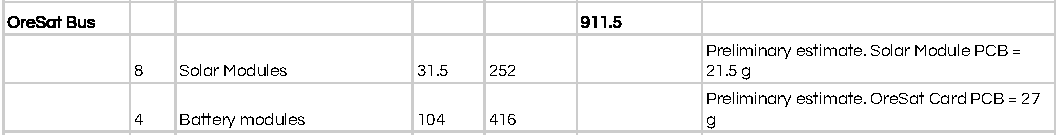
\includegraphics[width=\linewidth]{fig/eps-case-studies/oresat-mass-rows.pdf}
\caption[Published OreSat module mass estimates.]{Column headings and EPS rows reproduced (cropped) from the Portland State Aerospace Society's 2016 OreSat mass budget \citep[Sec.~D.2, p.~22]{oresat2016csli}. The source repository uses the \href{https://github.com/oresat/oresat.github.io/blob/0d879a503be4a6d48e849f3088524c2748503640/LICENSE}{GNU General Public License version 2}. The preliminary estimates give $8\times31.5=252$~g for solar modules and $4\times104=416$~g for battery modules. These are the external MOP-12 mass references. Occupied volumes are separate assessment assumptions.}
\label{fig:source-oresat-mass}
\end{figure}
\clearpage

\begin{figure}[p]
\centering
\small
\textbf{(a) Excerpt from the later OreSat solar description}\par\smallskip
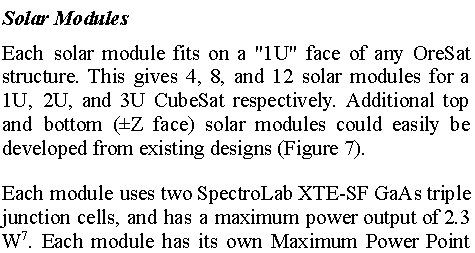
\includegraphics[width=0.76\linewidth]{fig/eps-case-studies/oresat-solar-configuration.pdf}
\par\smallskip
\textbf{(b) AZUR 3G30A electrical table}\par\smallskip
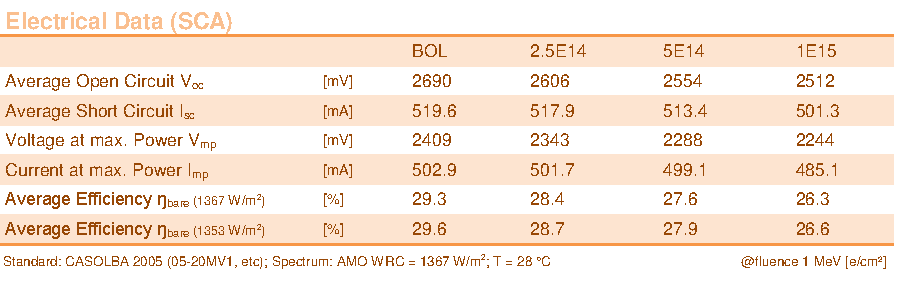
\includegraphics[width=\linewidth]{fig/eps-case-studies/azur-electrical-ratings.pdf}
\par\smallskip
\textbf{(c) Spectrolab XTE-SF electrical table}\par\smallskip
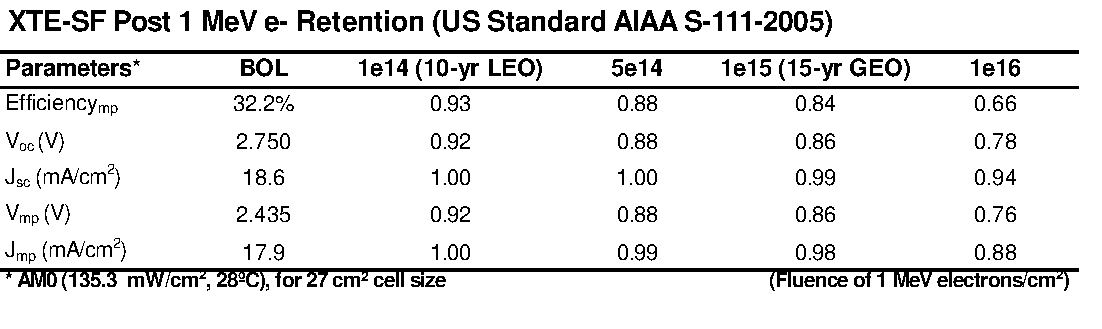
\includegraphics[width=\linewidth]{fig/eps-case-studies/spectrolab-electrical-ratings.pdf}
\caption[Original solar identities and condition-qualified ratings.]{Panel (a) is reproduced (cropped) from Greenberg et al., Portland State Aerospace Society at Portland State University \citep[p.~5]{greenberg2021oresat}, and identifies two XTE-SF cells per module. Panel (b) is reproduced (cropped) from AZUR SPACE Solar Power GmbH, copyright 2010 \citep[p.~2]{cots-mission_azur_space_3g30a_review_legacy_ds}. Panel (c) is reproduced (cropped) from Spectrolab Inc. \citep[p.~1]{cots-solar_src_spectro_xtesf}. The tables supply the independent MOP-11 MPP ratings and radiation variations. Their temperature, irradiance, area and fluence labels fix the scope of the comparison. Typical MPP values provide estimated power.}
\label{fig:source-solar-ratings}
\end{figure}
\clearpage

\begin{figure}[p]
\centering
\small
\textbf{(a) Original I--V plot and labels}\par\smallskip
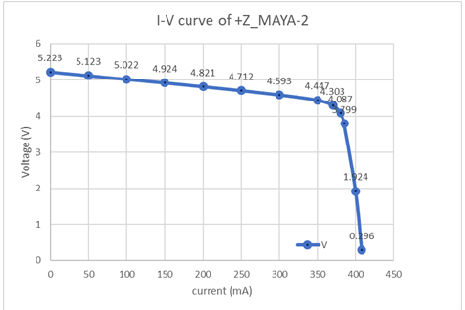
\includegraphics[width=0.85\linewidth]{fig/eps-case-studies/birds-iv-labels.pdf}
\par\smallskip
\textbf{(b) Original power plot and labels}\par\smallskip
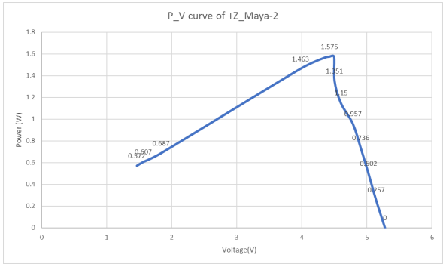
\includegraphics[width=0.85\linewidth]{fig/eps-case-studies/birds-pv-labels.pdf}
\caption[Published Maya-2 solar-characterization labels.]{Maya-2 plots reproduced (cropped) from Shrestha et al. \citep[Figs.~13--14, pp.~6--7]{shrestha2021birdssafety}. Copyright 2021 International Astronautical Federation. All rights reserved. MOP-18 compares $5.123~\mathrm{V}\times50~\mathrm{mA}=0.25615$~W with the 0.257~W label. The 0.331\% difference follows from the printed labels. The 1.575~W peak remains a separate published observation, without a reconstructed complete measured curve.}
\label{fig:source-birds-curves}
\end{figure}
\clearpage
